\section{Results}
\begin{figure}[h]
    \centering 
    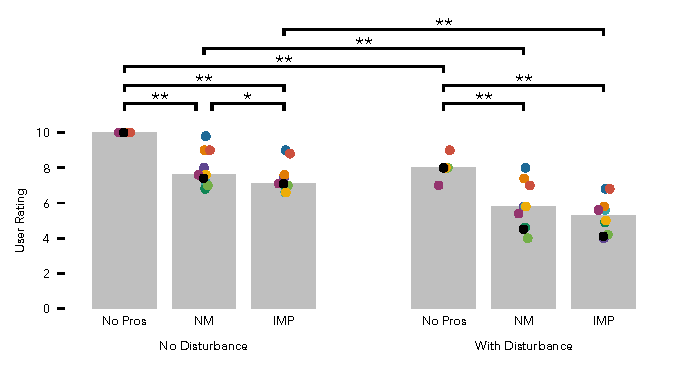
\includegraphics[width=\textwidth]{treadmill_vib_user_scores}
    \caption{Average user ratings across all trials in both the undisturbed and
    disturbed walking conditions when walking without the prosthesis (No Pros)
    and with the Neuromuscular (NM) prosthesis control and impedance (IMP)
    prosthesis control. Grey bars show the mean across subjects.  Statistical
    significance assessed by Welch's $t$-test. $*$:~$p < 0.05$, $**$:~$p <
    0.01$, $***$:~$p < 0.001$.}\label{fig:treadmill_user_ratings}
\end{figure}
First, \cref{fig:treadmill_user_ratings} shows the user ratings of the different
conditions. We mandated that users rate the No Prosthesis/No Disturbance case
10/10 so that other conditions could be rated relative to this case. We see that
in both the no disturbance and disturbance cases, neuromuscular control was
rated significantly more preferably than impedance control. Neither control
could match the ratings given to the no prosthesis case. Introduction of the
disturbance caused a significant drop in user rating for all controllers. 

\begin{figure}[t]
    \centering 
    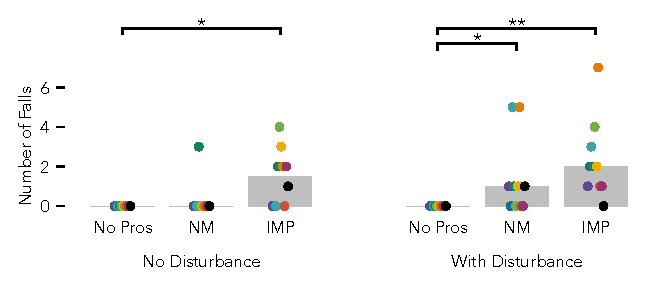
\includegraphics[width=\textwidth]{treadmill_vib_num_falls}
    \caption{Total number of falls across all trials in both the undisturbed and
    disturbed walking conditions when walking without the prosthesis (No Pros)
    and with the Neuromuscular (NM) prosthesis control and impedance (IMP)
    prosthesis control. Grey bars show the median number of falls across all
    subjects. Statistical significance assessed by Wilcoxon signed-rank test.
    $*$:~$p < 0.05$, $**$:~$p < 0.01$.}\label{fig:treadmill_exp_falls}
\end{figure}
Next, \cref{fig:treadmill_exp_falls} shows the number of falls in each
condition. Here we see that there was significant differences in the median
number of falls between impedance control and no prosthesis walking in the no
disturbance case and both impedance and neuromuscular walking in the disturbance
case. No significant differences were found directly between the neuromuscular
and impedance controllers.

\begin{figure}[b]
    \centering 
    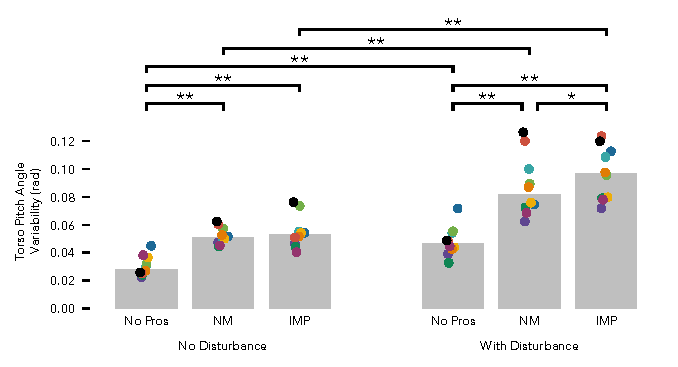
\includegraphics[width=\textwidth]{treadmill_vib_torso_var_x}
    \caption{Torso pitch angle variation. Angle variation calculated as the
    interquartile range of torso angles after the median torso angle trajectory
    over the strides in a trial is subtracted out. For the prosthesis trials, we
    report the average variation across the five trials for each condition.
    Grey bars show the mean across subjects.  Statistical significance assessed
    by Welch's $t$-test. $*$:~$p < 0.05$, $***$:~$p <
    0.001$.}\label{fig:treadmill_exp_torso_var_x}
\end{figure}

\begin{figure}[t]
    \centering 
    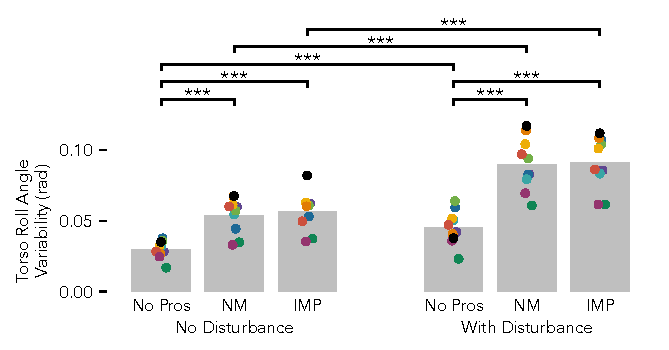
\includegraphics[width=\textwidth]{treadmill_vib_torso_var_y}
    \caption{Torso roll angle variation. Angle variation calculated as the inter
    quartile range of torso angles after the median torso angle trajectory over
    the strides in a trial is subtracted out. For the prosthesis trials, we
    report the average variation across the five trials for each condition.
    Grey bars show the mean across subjects.  Statistical significance assessed
    by Welch's $t$-test.$***$:~$p < 0.001$.}\label{fig:treadmill_exp_torso_var_y}
\end{figure}

\Cref{fig:treadmill_exp_torso_var_x,fig:treadmill_exp_torso_var_y} show the
torso pitch and roll angle variability respectively. We see significant
differences between the no prosthesis and with prosthesis cases as well as the
no disturbance and with disturbance cases. There is also a significant increase
in torso pitch variability with the impedance control compared to the
neuromuscular control in the disturbance case.

\begin{table}[t]
  \begin{center}
    \begin{tabular}{lcc}
      Fall Types & Neuromuscular & Impedance \\
      \midrule
      Fall Forward &  1 &  0 \\
      Fall Backwards &  6 &  4 \\
      Fall Left &  1 &  0 \\
      Fall Right &  0 &  3 \\
      Missed Stance / Swing Transition &  3 &  0 \\
      Missed Stance 2 / Stance 3 Transition &  0 &  7 \\
      Knee Collapse & 0 & 15 \\
      Swing Trip & 4 & 12 \\
    \end{tabular}
  \end{center}
  \caption{Tally of observed reasons for falls across all subjects and across
  both the undisturbed and disturbed walking conditions. Falls were manually
  classified based on video and logged prosthesis data. An individual Fall can
  be assigned more than one reason.}\label{tab:treadmill_exp_fall_reasons}
\end{table}
Finally, \cref{tab:treadmill_exp_fall_reasons} shows a tally of the reasons for
the observed falls with each controller type when using preferred parameters.
The reason for each fall was determined from analyzing video recordings and
logged prosthesis data. The first four categories refer to general losses of
balance resulting in a fall in the four cardinal directions. Backward falls
generally resulted from the treadmill suddenly stopping when the prosthesis
stance leg was still in front of the body, causing a loss of balance backwards.
The falls forward, left and right were generally more ambiguous in their cause,
but may be due to improper leg placement. 

The missed stance/swing transitions in the neuromuscular control were caused
when subjects did not allow the leg angle to cross the $90^\circ$ threshold set
in stance/swing state machine (compare \cref{fig:stance_swing_state_machine}).
The missed stance 2/stance 3 transitions occurred with impedance control if the
user did not dorsiflex the ankle sufficiently to trigger the transition. This
could cause the knee to produce an extension torque in late stance, making it
difficult to enter the swing phase (compare \cref{fig:treadmill_imp_fit}).

As shown in \cref{fig:treadmill_exp_phase_success}, the rate at which the
impedance conrtroller failed to transition through all three stance phases
significantly increased with the introduction of disturbances.
\begin{marginfigure}
    \centering 
    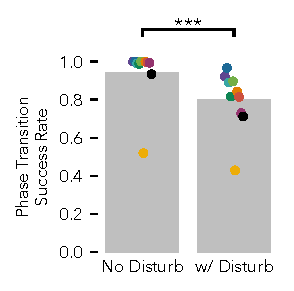
\includegraphics[width=\textwidth]{phase_success}
    \caption{Fraction of steps for which impedance control successfully
    transitions through all three stance phases. Introduction of gait
    disturbances significantly decreases the transition success rate. Grey bars
    show the mean success rate across all users. Statistical significance
    assessed by Welch's $t$-test. $***$:~$p <
    0.001$.}\label{fig:treadmill_exp_phase_success}
\end{marginfigure}

In contrast, the knee collapse fall type was triggered with impedance control if
the user dorsiflexed the ankle too early causing a premature switch to the third
phase of stance. In this phase, knee torque typically trends towards zero to
allow for passive flexion of the knee heading into swing. However, in the case
of a premature switch to the push-off phase, these near-zero knee torques can
cause the knee to suddenly collapse under the user's weight. 

The last cause of falls, trips during swing, occurred when using both
controllers, but 3x more often with impedance control than with neuromuscular
control. Many of the swing trips for impedance control were also preceded by a
missed stance 2/stance 3 transition. Others occurred when kinematics were
drastically changed by the disturbance. For example, several swing trips
occurred after a sudden acceleration of the treadmill caused the stance step
length to dramatically increase, thereby altering kinematics at toeoff and in
swing, and leading to the toe hitting the ground mid-swing.

\begin{figure}[b]
    \centering 
    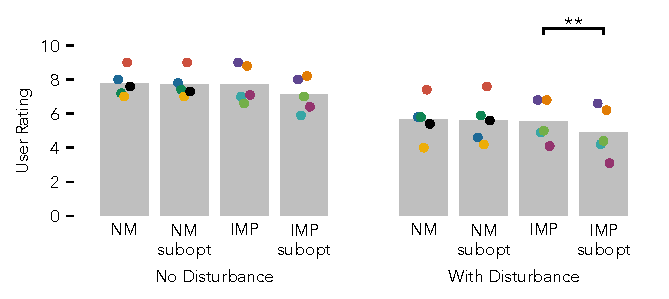
\includegraphics[width=\textwidth]{treadmill_vib_user_scores_subopt}
    \caption{Comparison of user scores of optimal versus suboptimal parameters
    for the neuromuscular and impedance control strategies. Grey bars show the
    mean user rating across subjects. Statistical significance assessed by
    Welch's $t$-test. $**$:~$p <
    0.01$.}\label{fig:treadmill_exp_user_ratings_subopt}
\end{figure}
Finally, we look at the effect of using suboptimal controllers on user ratings
and falls. \Cref{fig:treadmill_exp_num_falls_subopt} shows the median ratings of
each the preferred and suboptimal parameters for each controller. For
neuromuscular control, we see no significant difference between the preferred
controller from day 4 and the suboptimal controllers. In fact for the
neuromuscular control with disturbances, 4 out of 5 users slightly preferred the
suboptimal control from day 5. On the whole, choosing a suboptimal set of
parameters seemed to have a larger effect on impedance control with 4 out of 5
subjects preferring the optimal to suboptimal with out disturbances and all five
subjects preferring the optimal impedance parameters to the suboptimal
parameters in disturbed case.

\Cref{fig:treadmill_exp_num_falls_subopt} shows the median number of falls
garnered by optimal and suboptimal parameters. In the disturbance case we see a
increase in the median number of falls with the suboptimal paramete sets over
the preferred parameter sets. However this difference was not significant.

\begin{figure}[t]
    \centering 
    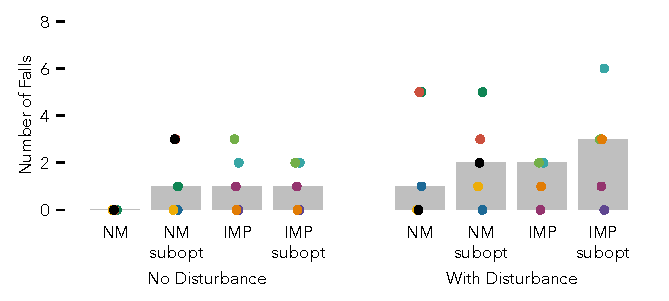
\includegraphics[width=\textwidth]{treadmill_vib_num_falls_subopt}
    \caption{Comparison of number of falls of optimal versus suboptimal
    parameters for the neuromuscular and impedance control strategies. Grey bars
    show the median number of falls across subjects. Statistical significance
    assessed by Wilcoxon signed-rank
    test.}\label{fig:treadmill_exp_num_falls_subopt}
\end{figure}
